\documentclass[zihao=false,fontset=windows]{ctexart}
% ctexart 不接受任意 pt 选项。正文改 {10pt}，方括号里是行距。
\usepackage{scrextend}
\changefontsizes[12pt]{10pt}

\usepackage[a4paper,left=2.35cm,right=2.35cm,top=1.7cm,bottom=1.9cm]{geometry}
\usepackage{xcolor}
\usepackage{graphicx}
\usepackage{amsmath,amssymb}
\usepackage{enumitem}
\usepackage{tabularx}
\usepackage{colortbl}
\usepackage{listings}
\usepackage{hyperref}
\usepackage[most]{tcolorbox}

\definecolor{feishuText}{RGB}{31,35,41}
\definecolor{feishuBlue}{RGB}{36,91,219}
\definecolor{feishuRed}{RGB}{216,57,49}
\definecolor{feishuGray}{RGB}{100,106,115}
\definecolor{feishuGray2}{RGB}{143,149,158}
\definecolor{feishuPinkBg}{RGB}{251,191,188}
\definecolor{quoteBar}{RGB}{51,112,255}
\definecolor{codebg}{RGB}{245,246,247}
\definecolor{codeborder}{RGB}{222,224,227}
\definecolor{inlinebg}{RGB}{242,243,245}
\definecolor{callRed}{RGB}{253,226,226}
\definecolor{callOrange}{RGB}{255,245,235}
\definecolor{callYellow}{RGB}{254,255,240}
\definecolor{callGreen}{RGB}{240,251,239}
\definecolor{callBlue}{RGB}{240,244,255}
\definecolor{callRedSoft}{RGB}{254,241,241}
\definecolor{callSun}{RGB}{255,255,204}
\definecolor{tableHead}{RGB}{242,243,245}
\definecolor{tableRule}{RGB}{222,224,227}
\definecolor{codeText}{RGB}{31,35,41}
\definecolor{codeKeyword}{RGB}{0,0,255}
\definecolor{codeComment}{RGB}{0,128,0}
\definecolor{codeString}{RGB}{163,21,21}

\setmainfont{Times New Roman}
\setCJKmainfont{Microsoft YaHei}[AutoFakeBold=2.2]
\setCJKsansfont{Microsoft YaHei}[AutoFakeBold=2.2]
\setCJKmonofont{Microsoft YaHei}[AutoFakeBold=2.2]
\setmonofont{Consolas}
\newfontfamily\emojifont{Segoe UI Emoji}

\hypersetup{
  colorlinks=true,
  urlcolor=feishuBlue,
  linkcolor=feishuBlue,
  unicode=true,
  pdftitle={BEiT-v3(2023, Microsoft)}
}

\setlength{\parindent}{0pt}
\setlength{\parskip}{0.42em}
\setlength{\fboxsep}{1.5pt}
\setlength{\emergencystretch}{3em}
\linespread{1.28}
\color{feishuText}
\arrayrulecolor{tableRule}
\urlstyle{same}

\setlist[enumerate]{label=\textcolor{feishuBlue}{\arabic*.}, leftmargin=1.7em, itemsep=0.22em, topsep=0.28em, parsep=0.08em, partopsep=0pt}
\setlist[itemize,1]{label=\textcolor{feishuBlue}{\textbullet}, leftmargin=1.35em, itemsep=0.18em, topsep=0.25em, parsep=0.06em, partopsep=0pt}
\setlist[itemize,2]{label=\textcolor{feishuBlue}{◦}, leftmargin=1.45em, itemsep=0.12em, topsep=0.15em}
\setlist[itemize,3]{label=\textcolor{feishuBlue}{\rule[0.18em]{0.38em}{0.38em}}, leftmargin=1.55em, itemsep=0.1em, topsep=0.12em}

\newcommand{\feiEmoji}[1]{{\emojifont #1}}
\newcommand{\incode}[1]{\colorbox{inlinebg}{\ttfamily\small #1}}
\newcommand{\bigmath}[1]{%
  \begin{center}\large$\displaystyle #1$\end{center}%
}
\newcommand{\rb}[1]{\textcolor{feishuRed}{\textbf{#1}}}

\lstset{
  language=Python,
  basicstyle=\ttfamily\footnotesize\color{codeText},
  keywordstyle=\color{codeKeyword},
  commentstyle=\color{codeComment},
  stringstyle=\color{codeString},
  showstringspaces=false,
  breaklines=true,
  columns=fullflexible,
  keepspaces=true,
  tabsize=4,
  upquote=true,
  aboveskip=2pt,
  belowskip=0pt,
  xleftmargin=0pt,
  frame=none
}

\tcbset{
  feishubase/.style 2 args={
    enhanced,
    boxrule=0pt,
    arc=8pt,
    left=10pt,
    right=10pt,
    top=7pt,
    bottom=7pt,
    before skip=6pt,
    after skip=6pt,
    colback=#1,
    colframe=#1,
    before upper={\feiEmoji{#2}\hspace{0.45em}\ignorespaces}
  }
}
\newtcolorbox{feishubox}[2]{feishubase={#1}{#2}, breakable}
\newtcolorbox{feishuboxnb}[2]{feishubase={#1}{#2}}

\newtcolorbox{feishuquote}{
  enhanced,
  breakable,
  boxrule=0pt,
  leftrule=3pt,
  arc=0pt,
  colframe=quoteBar,
  colback=white,
  left=8pt,
  right=2pt,
  top=2pt,
  bottom=2pt,
  before skip=4pt,
  after skip=4pt,
  before upper=\color{feishuGray}
}

\newtcolorbox{feishucode}{
  enhanced,
  breakable,
  colback=codebg,
  colframe=codeborder,
  boxrule=0.6pt,
  arc=6pt,
  left=6pt,
  right=6pt,
  top=5pt,
  bottom=4pt,
  before skip=6pt,
  after skip=6pt
}

\begin{document}
{\zihao{1}\bfseries BEiT-v3(2023, Microsoft)\par}

\begin{feishuquote}
BEiT-v3：大一统(2023, Microsoft)\par
\href{https://arxiv.org/abs/2208.10442}{Image as a Foreign Language: BEiT Pretraining for All Vision and Vision-Language Tasks}\par
\end{feishuquote}

不论是在Language、Vision还是在多模态领域，Big Convergence是大势所趋。\par

\begin{feishuquote}
也就是在超大的数据集上做大规模的预训练，一旦模型训练好之后，它的特征就已经非常好了，可以直接Transfer到下游任务上去，尤其是当模型足够大、数据足够多的时候，有可能预训练出来一个有通用性能的Foundation Model，这个Foundation Model能解决各种的模态或者各种下游任务，非常的强大。\par
\end{feishuquote}

相比之前的多模态模型如CLIP和CoCa，\rb{BEiT-v3 的关键词就是：Big Convergence 大一统}，即：\rb{将图像看成一种“语言”}，用一个模型架构和一个训练任务，打造出多模态领域的集大成者，\textbf{统一多模态学习中的模型结构、预训练任务以及模型规模}。\par

A big convergence of language, vision, and multimodal pretraining is emerging，即视觉的表征，语言的表征和多模态的表征都在大一统。BEiT-v3 使用 Transformer 模型统一处理视觉和文本信息，使用Mask Data Modeling的训练策略统一建模视觉和文本信息。\par

BEiT-v3从三个方面实现了大一统：\par
\begin{itemize}
\item \rb{模型架构 Multiway Transformer}
\begin{itemize}
\item 其实就是VLMo中MoME
\item 统一输入形式（将图像看作是一种“语言”），\textbf{文本 English、图像 Imaglish、图文对 Parallel Sentences}
\end{itemize}
\item \rb{预训练任务 Mask Data Modeling}
\begin{itemize}
\item 输入形式统一之后，也就不需要 ITC、ITM、MLM等其他目标函数，可以使用\textbf{统一的 mask “language” modeling 的方式进行训练}
\end{itemize}
\item \rb{模型scaling up (将模型放大)}
\begin{itemize}
\item 模型扩大到了ViT-giant的配置，参数量达到了1.9B (vision/language各一半），提升多模态效果
\end{itemize}
\end{itemize}

\par\vspace{1.15em}\noindent{\zihao{-2}\bfseries 1. 模型架构}\par\vspace{0.28em}

\begin{feishuquote}
从模型角度来说，Transformer非常关键：\par
\begin{itemize}
\item \textbf{Transformer框架相比CNN的优势}：未来肯定是多模态的，一个模型做所有的Modality，所有的Task，肯定是一个大一统的框架。但是CNN不太适合做其他的Modality，而Transformer就适合做很多的Modality。从这一点上对比Transformer就胜出了。
\item \href{https://scnajei2ds6y.feishu.cn/wiki/WhjkwoywXi5QN9kfeXaciiABnvb}{VLP常用框架}：Dual Encoder、Encoder-Decoder、Fusion Encoder三种框架，这个在前面介绍过。
\end{itemize}
不论是哪种方式，这些模型在遇到下游任务的时候，因为输入的形式可能会改变或者输出的形式有时候会改变，所以模型需要根据下游任务去做一些改进，因此不是真正意义上的General Purpose Modeling。\par
\end{feishuquote}

所以，BEiT-v3采用的是VLMo中使用的\href{https://scnajei2ds6y.feishu.cn/wiki/Dab8wydhtii0tpk1RXvcMJ8Vnoc\#D2ZHdsB0uovW6Xx6TbOcfukpnXg}{\textbf{MoME}}（Mixture-of-Modality-Experts），这里改了个名字叫 \textbf{Multiway Transformer。}\par

\begin{center}
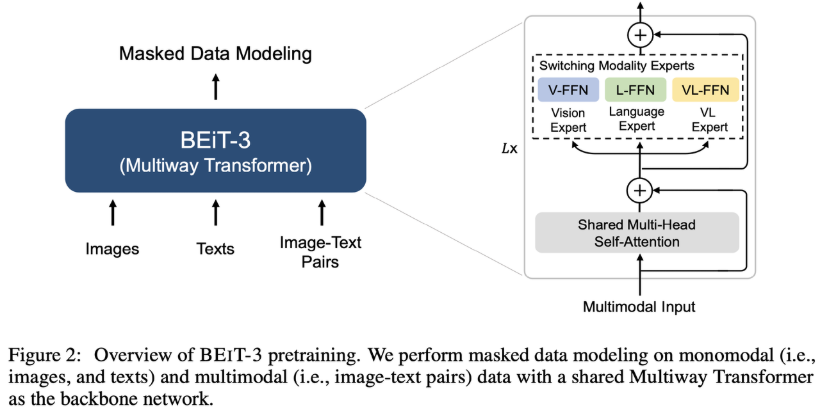
\includegraphics[width=0.98\textwidth]{images/2023-CVPR-BEiT-v3/fig-01.png}
\end{center}

BEiT-v3 预训练一个模型，通过模块化的搭积木，就可以灵活处理各种下游任务（每一个训练好的Transformer Block、SA层、FFN都可以随意的拼装和组合）。\par

\begin{center}
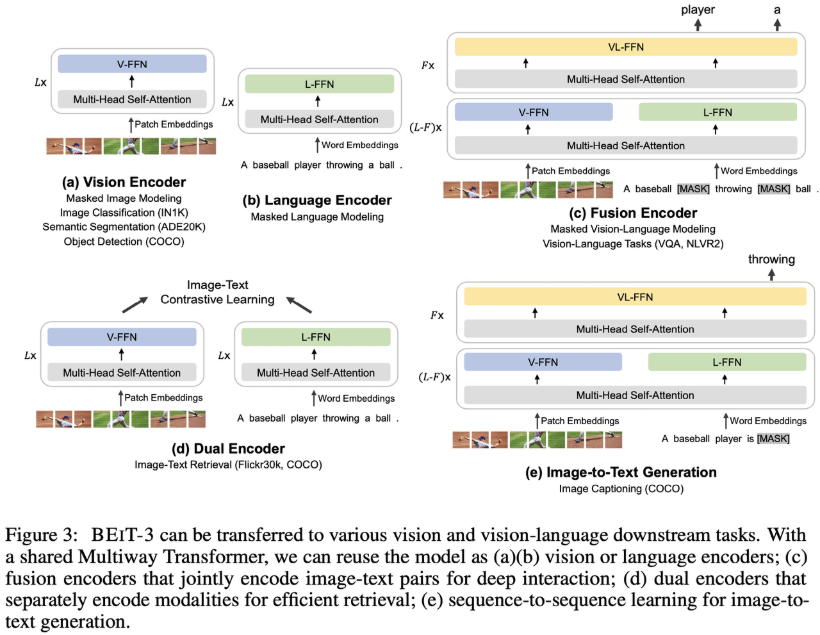
\includegraphics[width=0.98\textwidth]{images/2023-CVPR-BEiT-v3/fig-02.png}
\end{center}

输入的数据根据模态的不同选择不同的 Expert，比如图片数据就使用 Vision FFN，文本数据就使用 Language FFN。模型前面的一些层是只有 Vision FFN 和 Language FFN，到了最后3层为了特征融合会再有 Vision-Language FFN。\par
\begin{itemize}
\item 图中(a) 所示是 BEiT-v3模型转换为视觉编码器，适配任务：图像分类，目标检测，语义分割；
\item 图中(b) 所示是 BEiT-v3模型转换为文本编码器；
\item 图中(c) 所示是单塔结构，联合编码图像-文本对以进行深度交互的融合编码器，适配任务：多模态理解任务 ；
\item 图中(d) 所示是双塔结构，对每个模态进行单独编码以求高效的图文检索，适配任务：图文检索任务 ；
\item 图中(e) 所示是单塔结构，用于图像到文本生成任务，适配任务：多模态生成任务 。
\end{itemize}

\textcolor{feishuBlue}{但是有人觉得 BEiT-v3 还不能算是 foundation model，因为它只是设计了比较精妙的 block，像搭积木一样做了排列组合。当时已经有人觉得应该用 language 作为 interface 将所有的任务统一起来，LLM 出现之后我们离这样的目标更近了一步。}\par

\par\vspace{1.15em}\noindent{\zihao{-2}\bfseries 2. 预训练任务}\par\vspace{0.28em}

文本中以BERT为代表的\href{https://scnajei2ds6y.feishu.cn/wiki/U5sZwCwKwivERwktFWvcdM50nkf\#C7YrdlkjHoRWhVxE5BicV7xNnjJ}{MLM} + 视觉中以BEiT为代表的\href{https://scnajei2ds6y.feishu.cn/wiki/Dab8wydhtii0tpk1RXvcMJ8Vnoc\#GaUYdY7iVo8Qtexy6CEc6XaGn3f}{MIM}，这两种Mask Data Modeling（MDM）预训练方式已经取得了成功。\par

BEiT-v3，将MDM扩展到多模态领域，进一步将所有多模态数据都看作是一种“语言”，以此统一预训练：\par
\begin{itemize}
\item \textbf{文本 English}
\item \textbf{图像 Imaglish （}Image + English造出来的词，Sequence of Token）
\item \textbf{图文对 Parallel Sentences}（双语句对，句子1后面跟了个句子2）
\end{itemize}

\begin{feishubox}{callSun}{🙋}
\rb{为什么要统一预训练方式？}\par
\begin{itemize}
\item \textbf{MDM 已经广泛应用在}文本、图像、图文中，表明 MDM 作为一个目标函数已经可以很好地学习文本、图像和多模态特征。
\item \textbf{用一个 loss 代替多个 loss 可以降低复杂度：}
\begin{itemize}
\item 传统方法会用 ITM（Image-Text Matching）、ITC（Image-Text Contrastive）等多个损失函数，但这会带来：
\par
\textbf{计算效率低}：大模型和大数据集下计算成本高
\par
\textbf{调参难度大}：多个 loss 需要调整、平衡权重，有些 loss 可能互补，有些可能互斥
\par
\textbf{人工调参难以 scale up}：比如 ITM 需要 ITC 先找 hard negative，再做匹配，整个流程复杂
\end{itemize}
\item \textbf{MDM更有助于开展自监督学习}
\end{itemize}
\end{feishubox}

MDM的具体方法：\par
\begin{itemize}
\item 文本数据：由 SentencePiece tokenizer 进行token化
\item 图像数据：由 BEiT-v2 的 tokenizer 进行token化，变成Sequence of Token
\item 具体mask方法：还是原来的MLM、MIM中的mask方法，从单模态文本中随机 mask 掉 15\% 的文本，从图片-文本对中随机 mask 掉 50\% 的文本，在 mask 图像时采用 block-wise 掩码策略 mask 掉 40\%。
\item 预训练目标：还是一样做完形填空，恢复掉被遮住的图像或文本。
\end{itemize}

\par\vspace{1.15em}\noindent{\zihao{-2}\bfseries 3. 模型放大}\par\vspace{0.28em}

Scaling up是提高基础模型的泛化质量的有效方法，更有效的将模型转移到各种下游任务中。（因为只有用了更多的数据，有一个容量很大的模型，它才有可能用一个模型去解决所有的事情）\par

BEiT-v3将模型大小扩展到\textbf{Billions of Parameters}，数据集（\textbf{开源}）也扩展到非常大。\par

\begin{feishubox}{callSun}{🙋}
\rb{为什么 BEiT-3 可以轻松扩展模型规模？}\par
因为它使用了\textbf{单一的 MDM预训练目标}，从而避免了传统对比学习方法在批量大小（batch size）和计算资源上的挑战。\par
\begin{itemize}
\item 只使用MDM，可以避免对比学习的Batch Size限制
\par
\textbf{对比学习的痛点}：
\begin{itemize}
\item 需要\textbf{极大的 batch size} 才能保证模型学习到有意义的表示，因为它依赖\textbf{正负样本对比}。
\item \textbf{显存和通信开销巨大}，使得在大模型上训练非常困难，需要大量工程优化。
\item 如果 batch size 变小，对比学习的效果会显著下降，使得扩展模型变得更加困难。
\end{itemize}
\par
\textbf{BEiT-v3 的优势}：
\begin{itemize}
\item 只使用 \textbf{MDM} 作为唯一的预训练任务，不依赖 batch 内样本的对比关系，因此 batch size 可以自由调整，而不会影响模型性能。
\item \textbf{不再受 batch size 限制}，意味着可以更高效地训练更大的模型。
\end{itemize}
\item 无 Batch 内依赖，适合梯度累积
\begin{itemize}
\item 传统对比学习方法需要在 batch 内对不同样本进行计算，无法轻松使用梯度累积。
\item \textbf{BEiT-v3 由于只用 MDM，没有 batch 内部的交互依赖，天然适用于梯度累积}，可以高效训练超大规模模型。
\end{itemize}
\item 可以直接借鉴 LLM 的 Scaling Up 经验
\begin{itemize}
\item 由于 BEiT-3 采用 MDM，训练方式与 NLP 任务（如 BERT、GPT）类似，可以\textbf{直接复用语言模型的 Scaling Up 经验}。
\end{itemize}
\end{itemize}
\end{feishubox}

\par\vspace{1.15em}\noindent{\zihao{-2}\bfseries 4. 总结}\par\vspace{0.28em}

BEiT-v3其实从方法上来说就是之前BEiT、BEiT-v2、VL-BEiT、VLMo等一系列的工作的一个集合体，本身没有提出新的内容，主要就是把它做大做强，展示了一个Unified Framework能达到的性能。\par

\textbf{到这里时，其实已经呈现了一个趋势，多模态模型的规模在不断扩大，训练用的数据规模也在扩大，虽然一定程度上对性能有利的，但是端到端训练的成本也会随之增加。}\par

\textbf{此时也就会有另外一种思考，有没有什么高效的对齐方法，直接利用已经预训练好的视觉、文本模型就能快速对齐，完成对模态任务。BLIP2就进行了验证。}\par

\end{document}
